
\documentclass{res} % This file uses the resume document class (res.cls)
\usepackage{helvetica}
\usepackage{newcent}    
\usepackage{graphicx}
\usepackage[usenames,dvipsnames]{color}
\definecolor{grey}{RGB}{211,211,211}


\setlength{\textheight}{9.5in} 
\setlength{\textwidth}{6.5in} 

\begin{document} 

\name{ KUNALKUMAR B CHAVDA\\[20pt]}    
				             

\address{\bf  ADDRESS\\1136, Himmat lal ni chali\\Opp. Bnak of Baroda\\Po. Bajwa\\Vadodara\\Gujarat-391310\\}
\address{\bf CONTACT \\ \textbf{Mo.} : +91 7874900739 \\  \textbf{E-m@il}: kunalchavda96@gmail.com}
\begin{figure}
{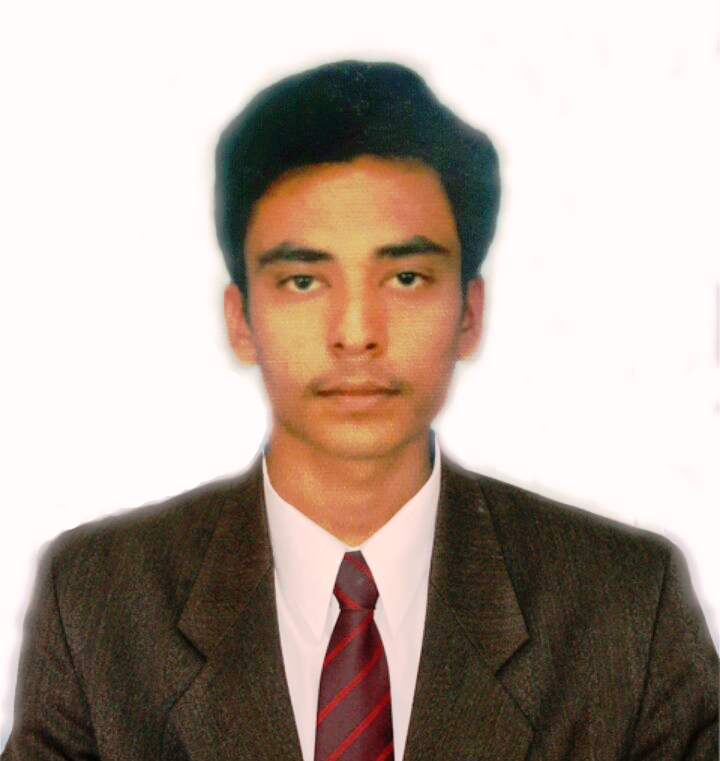
\includegraphics[width=3cm]{DSCN4570.JPG}}
\end{figure}

\begin{resume}

\section{
\colorbox{grey}{OBJECTIVE}
   }   
\ To work with well established technical organization for enhancement of my skills and betterment of future
 

\section{
\colorbox{grey}{EDUCATION}  
}
\begin{itemize}
\item Pursuing 8th Semester Bachelor of Engineering ( Civil Engineering )
\end{itemize}    

\begin{table}[ht] 
 \centering% used for centering table
\begin{tabular}{||c|c|c|c|c||} % centered columns (5 columns)
\hline
\hline\\ [.5ex] %inserts double horizontal lines
EXAMINATION & UNIVERSITY & INSTITUTE & YEAR & RESULT/CGPA \\ [.5ex] % inserts table
\hline
\hline\\ [.5ex]
BE SEM-7 & GTU & Vadodara Institute of Engg. & 2018 & 7.08 \\ [.5ex] % inserting body of the table
HSC & GSHSEB & Fertilizer Nagar Schhol & 2013 & 55.1{\%} \\ [.5ex] 
SSC & GSEB & Mahireva Aadarsh Vidyalaya & 2011 & 81.4{\%} \\ [1ex]
\hline %inserts single line 
\end{tabular}
\label{table:lin} % is used to refer this table in the text
\end{table}




\section{
\colorbox{grey}{PROJECTS}
}

\begin{tabular}{ l l}
\ Name &  {:} \textbf{Restoration and replenishment of tributaries of Vishwamitri river}\\ [0.5ex]
\ During & {:}  \textbf{7th and 8th semester} \\ [0.5ex]
\ Applocation  &  {:} \bf RIVER RESTORATION  \\ [0.5ex]
\ Summary & {:} \\
\end{tabular}

%-------------------------------------------------------
\             The filter is used to restore and rehabilitate tributaries of any river by filtering waste water coming from upstream side of a tributary and discharging treated water to the river. Filter is designed that it can operate itself or can be operated manually under the supervision of single operator. The filter also designed keeping in mind flooding conditions and its relative measures are manipulated by micro-controller. In high flood condition, filter will get lifted so that it does not become an obstruction to the flood flow and surrounded area will not be affected. This type of portable filter can be for any tributary of river to reduce overall polution load of river.  \par
%-------------------------------------------------------

\section{
\colorbox{grey}{TRAINING/INTERNSHIP}
}
\begin{itemize}
\item Attended workshop on “Use of Microsoft Excel in Civil Engineering” organized by EZ Professional Training Institute
\end{itemize}   


\section{
\colorbox{grey}{TECHNICAL SKILLS}       
}   
 \begin{itemize} 
 \item Simulations in Proteus-ISIS
 \item Arduino Programming
 \item MS-Excel based calculation sheets 
\item Adobe PhotoShop
\item Basics of electrical {\&} electronic components
\item Knowlegde of surveying equipments

 \end{itemize}

 
\section{
\colorbox{grey}{SOFT SKILLS}          
}
    \begin{enumerate} 
 \item Good problem solving ability with dynamic thinking
 \item Open minded to work in projects and team work
 \item Good Presentation skills
 \item Good Grasping Power
 \item Leadership
 \end{enumerate}


\section{
\colorbox{grey}{EXTRACURRICULAR ACTIVITIES}          
}
\begin{itemize} 
 \item Participated in GTU TECHFEST 2014
 \item Participated in 12th ISTE state annual student convention 2015
 \item Secured 2nd Rank in National Environment Awareness Campaign 2014-15
 \item Participated in Environment Awareness Campaign 2016-17
 \item Secured 1st Rank in Roller costal and Paper Sky scrapper events, \textbf{VIEROTSAV} held at Vadodara Institute of Engineering 2017
 \item Awarded as Most Innovative Sollution in \textbf{E- Yantra Ideas Competition} held at IITB 2018
 \item Secured 1st Rank in \textbf{TechEureka} event held at G H Patel Collage of Engineerin and Technology (GCET), V.V. Nagar
 \end{itemize}


\section{
\colorbox{grey}{CO-CURRICULAR ACTIVITIES} 
}         
\begin{enumerate} 
 \item Contour Survay at \textbf{Tajpura Village}
 \item Visited to \textbf{ Water Treatment Plant and Effluent Treatment Plant, Vadodara}
\item Visited to \textbf{ Gujarat Engineering Research Institute, Vadodara}
\item Visited to \textbf{ National Academy of Indian Railways, Vadodara }
 \end{enumerate}


\section{
\colorbox{grey}{HOBBIES}
}
\begin{itemize}
\item Travelling
\item Listening songs, watching movies, Drama
\item Playing Cricket, Football, Basketball and Volleyball on weekends
\item Programing and gaming
\end{itemize}


\section{
\colorbox{grey}{PERSONAL DETAILS} 
}
\ \\ [0.5ex]
\begin{tabular}{p{4cm}l}
\textbf{Father's Name} &  {:} Bhagwansinh C Chavda\\ [0.5ex]
\textbf{Mother's Name} & {:}  Manjulaben B Chavda \\ [0.5ex]
\textbf{Sex} &  {:} Male\\ [0.5ex]
\textbf{Date of Birth} & {:} 11 August 1996\\ [0.5ex]
\textbf{Nationality} &  {:} Indian\\ [0.5ex]
\textbf{Marital Status} & {:}  Unmarried\\ [0.5ex]
\end{tabular}







\end{resume}
\end{document}
